%        File: main.tex
%     Created: Thu Jul 01 07:00 AM 2010 U
% Last Change: Thu Jul 01 07:00 AM 2010 U
%
\documentclass[a4paper,10pt]{article}
\addtolength{\hoffset}{-2cm}
\addtolength{\voffset}{-1.25cm}
\addtolength{\textwidth}{4cm}
\addtolength{\textheight}{2.5cm}
\addtolength{\footskip}{-35pt}
\usepackage{amsmath,amsthm,amssymb}
\usepackage{url}
\usepackage{hyperref}
\usepackage{xtab}
\usepackage{multirow}
\usepackage{graphicx}
\usepackage{array}	
\usepackage{fancyhdr}
\begin{document}
\fancyhf{}
\renewcommand{\headrulewidth}{0pt}
\renewcommand{\footrulewidth}{1pt}
\renewcommand\footrule{\begin{minipage}{1\textwidth}
\hrule width \hsize height 2pt \kern 1mm \hrule width \hsize   
\end{minipage}\par}
\pagestyle{fancy}
\lfoot{April, 2013}
\cfoot{Ruihong Huang}
\rfoot{Page \thepage\ of 2}
\begin{tabular}[h]{p{0.3\textwidth}p{0.6\textwidth}}
  \vfill\hspace{-10pt}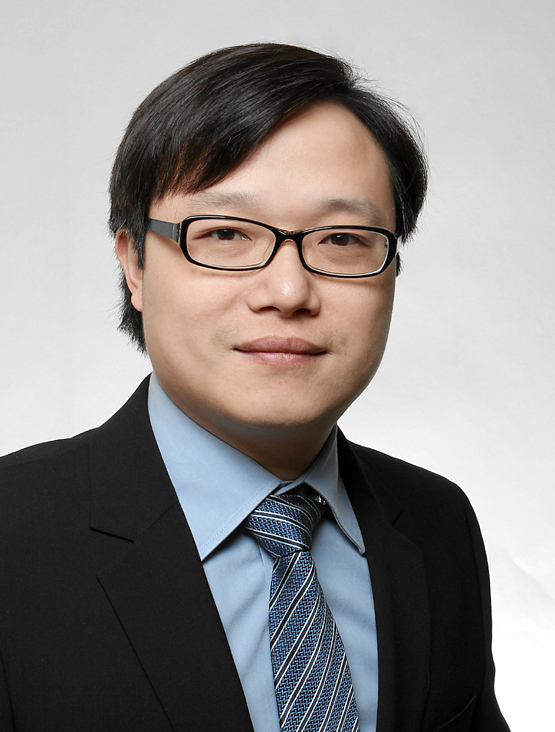
\includegraphics[width=0.3\textwidth]{bew/ruihong_2013.jpg} &\vspace{1pt}\large{\textbf{Dr. Huang, Ruihong}\newline 
Humboldt Universit\"at zu Berlin \newline 
Institute for Statistics and Econometrics  ­\newline
Spandauer Str. 1  \newline
10178 Berlin, Germany \newline
Tel: +49 30 2093 1459 \newline
Email: \verb|ruihong.huang@wiwi.hu-berlin.de| } \\
\end{tabular}\\
\rule[5pt]{1\textwidth}{1pt}\par
\setlength{\tabcolsep}{10pt}
\setlength{\extrarowheight}{6pt}
\begin{xtabular}[h]{p{0.15\textwidth}p{0.75\textwidth}}
  PROFESSIONAL\newline POSITIONS / \newline PRACTICAL \newline EXPERIENCE 
  & \textbf{Postdoc} \hfill 02/2012 -- present \newline Humboldt Universit\"at zu Berlin \hfill Berlin, Germany\newline Institute for Statistics and Econometrics \newline \emph{--Research on high-frequency trading and hidden liquidity in equity markets.} \\
  & \textbf{(External) Scientific Employee} \hfill 02/2008 -- 07/2011 \newline Deutsche Bank \hfill Berlin, Germany\newline Quantitative Products Laboratory\newline \emph{-- Research on econometric models for the limit order book and the order flow.} \\
  & \textbf{Consultant} \hfill 06/2002 -- 09/2003 \newline Ruling Consulting Co.\hfill Fuzhou, China \newline\emph{-- Advising Chinese mainland enterprises on the IPO procedure in the Hong Kong Exchanges.} \\
  & \textbf{Investment Analyst} \hfill 10/1998 -- 05/2002 \newline Hydro-Power Exploitation Co.\hfill Quanzhou, China \newline\emph{--Evaluating state’s investment in the hydro-power industry.} \newline\\
EDUCATIONS
  & \textbf{Doctorate in Econometrics} \hfill 02/1998 -- 02/2012 \newline Humboldt Universit\"at zu Berlin \hfill Berlin, Germany \newline Institute for Statistics and Econometrics\newline\emph{-- The econometric analysis on the high frequency order data.} \\
  & \textbf{Master student in Applied Math.} \hfill 09/2006 -- 02/2008 \newline Royal Inst. of Tech. (KTH) \hfill Stockholm, Sweden\newline School of Computer Science and Communication \newline\emph{-- Studies in numerical methods and the high-performance computation.} \\
  & \textbf{M.Sc. in Economics} \hfill 04/2004 -- 12/2007 \newline University of Copenhagen \hfill Copenhagen, Denmark  \newline Department of Economics \newline\emph{-- Studies in financial economics.}\\
  & \textbf{B.E. in Computer Applications} \hfill 09/1996 -- 07/1998 \newline Hohai University \hfill Nanjing, China \newline\emph{-- Studies in software design for industrial management.}\\
  & \textbf{B.M. in Management Engineering} \hfill 09/1993 -- 07/1997 \newline Hohai University \hfill Nanjing, China \newline\emph{-- Studies in the material management and delivery system.}\newline\\
\end{xtabular}\\\newline
\begin{xtabular}[h]{p{0.15\textwidth}p{0.75\textwidth}}
  COMPUTER \newline SKILLS &\vspace{-10pt}
   \begin{tabular}[t]{|p{0.18\textwidth}|p{0.40\textwidth}|c|}\hline
    Classfication & Details & Years\\ \hline
    Software\newline Development & LOBSTER \newline http://lobsterdata.com & 3 \\ \hline
    OS & Gentoo/Debian/Redhat Linux & 8 \\ \hline
    Programming  & C++, Java & 7 \\ \cline{2-3}
    Languages    & Python, SQL, KDB+ & 3 \\ \hline
    C++ Libraries& STL, OpenMP, MPI & 1.5 \\ \hline
    Math Software& Matlab, R        & 7 \\ \hline
  \end{tabular} \\
  &\\
  PUBLICATIONS\newline AND \newline RESEARCHES
  &\vspace{-20pt}
  \begin{enumerate}
    \item Hautsch, N. and R. Huang (2012), ``The market impact of a limit order'', Journal of Economic Dynamics and Control, 36, 501 – 522.
    \item  Hautsch, N. and R. Huang (2012), ``Limit order flow, market impact and optimal order sizes: Evidence from NASDAQ TotalView-ITCH data'' in: ``Market Microstructure: Confronting Many Viewpoints'', F. Abergel, J.-P. Bouchaud, T. Foucault, C. Lehal, M. Rosenbaum (eds.), Wiley Intersciences.
    \item Hautsch, N. and R. Huang (2012), ``On the dark side of the market: Identifying and analyzing hidden order placements'' Discussion Paper 2012-4, CRC 649, Humboldt University of Berlin.
    \item  Huang, R. and T. Xiao (2012), ``How much can hidden liquidity improve the trading price'' Working Paper, Humboldt University of Berlin and Harvard University.
    \item Huang, R. and T. Polak (2011), ``LOBSTER: Limit order book reconstruction system'' Working Paper, Humboldt University of Berlin.
    \item ``The impact of public news on the limit order flow'', Ongoing research with A. Gro\ss-Klu{\ss}mann (Humboldt University of Berlin).
    \item ``Does the circuit breaker help stabilizing the market'', Ongoing research with N. Hautsch (Humboldt University of Berlin).
    \item ``Does the hidden liquidity harm the price discovery'', Ongoing research with H. Zhu (MIT).
    \item ``Reinforcement learning on the optimal trading strategy with limit order books'', Ongoing research with Y. Sun (Technical University of Berlin).
  \end{enumerate}\\
  TEACHING&\vspace{-20pt}\begin{enumerate}
    \item Advanced Econometrics, 2012
    \item Seminar Econometric Projects, 2010\newline
  \end{enumerate}
\end{xtabular}
\end{document}
